\iffalse
This file is protected by Copyright. Please refer to the COPYRIGHT file
distributed with this source distribution.

This file is part of OpenCPI <http://www.opencpi.org>

OpenCPI is free software: you can redistribute it and/or modify it under the
terms of the GNU Lesser General Public License as published by the Free Software
Foundation, either version 3 of the License, or (at your option) any later
version.

OpenCPI is distributed in the hope that it will be useful, but WITHOUT ANY
WARRANTY; without even the implied warranty of MERCHANTABILITY or FITNESS FOR A
PARTICULAR PURPOSE. See the GNU Lesser General Public License for more details.

You should have received a copy of the GNU Lesser General Public License along
with this program. If not, see <http://www.gnu.org/licenses/>.
\fi

%----------------------------------------------------------------------------------------
% Required document specific properties
%----------------------------------------------------------------------------------------
\def\comp{backpressure}
\edef\ecomp{backpressure}
\def\Comp{Back Pressure}
\def\docTitle{\Comp{} Component Data Sheet}
\def\snippetpath{../../../../../doc/av/tex/snippets/}
%----------------------------------------------------------------------------------------
% Global latex header (this must be after document specific properties)
%----------------------------------------------------------------------------------------
\iffalse
This file is protected by Copyright. Please refer to the COPYRIGHT file
distributed with this source distribution.

This file is part of OpenCPI <http://www.opencpi.org>

OpenCPI is free software: you can redistribute it and/or modify it under the
terms of the GNU Lesser General Public License as published by the Free Software
Foundation, either version 3 of the License, or (at your option) any later
version.

OpenCPI is distributed in the hope that it will be useful, but WITHOUT ANY
WARRANTY; without even the implied warranty of MERCHANTABILITY or FITNESS FOR A
PARTICULAR PURPOSE. See the GNU Lesser General Public License for more details.

You should have received a copy of the GNU Lesser General Public License along
with this program. If not, see <http://www.gnu.org/licenses/>.
\fi

% Sets OpenCPI Version used throughout all the docs. This is updated by
% scripts/update-release.sh when a release is being made and must not
% be changed manually.
\def\ocpiversion{v2.2.0}

\documentclass{article}
\author{}  % Force author to be blank
\date{OpenCPI Release:\ \ \ocpiversion}  % Force date to be blank and override date with version
\title{OpenCPI\\\docTitle}  % docTitle must be defined before including this file
%----------------------------------------------------------------------------------------
% Paper size, orientation and margins
%----------------------------------------------------------------------------------------
\usepackage{geometry}
\geometry{
  letterpaper,  % paper type
  portrait,     % text direction
  left=.75in,   % left margin
  top=.75in,    % top margin
  right=.75in,  % right margin
  bottom=.75in  % bottom margin
}
%----------------------------------------------------------------------------------------
% Header/Footer
%----------------------------------------------------------------------------------------
\usepackage{fancyhdr} \pagestyle{fancy}  % required for fancy headers
\renewcommand{\headrulewidth}{0.5pt}
\renewcommand{\footrulewidth}{0.5pt}
\lhead{\small{\docTitle}}
\rhead{\small{OpenCPI}}
%----------------------------------------------------------------------------------------
% Various packages
%----------------------------------------------------------------------------------------
\usepackage{amsmath}
\usepackage[page,toc]{appendix}  % for appendix stuff
\usepackage{enumitem}
\usepackage{graphicx}   % for including pictures by file
\usepackage{hyperref}   % for linking urls and lists
\usepackage{listings}   % for coding language styles
\usepackage{pdflscape}  % for landscape view
\usepackage{pifont}     % for sideways table
\usepackage{ragged2e}   % for justify
\usepackage{rotating}   % for sideways table
\usepackage{scrextend}
\usepackage{setspace}
\usepackage{subfig}
\usepackage{textcomp}
\usepackage[dvipsnames,usenames]{xcolor}  % for color names see https://en.wikibooks.org/wiki/LaTeX/Colors
\usepackage{xstring}
\uchyph=0  % Never hyphenate acronyms like RCC
\renewcommand\_{\textunderscore\allowbreak}  % Allow words to break/newline on underscores
%----------------------------------------------------------------------------------------
% Table packages
%----------------------------------------------------------------------------------------
\usepackage[tableposition=top]{caption}
\usepackage{float}
\floatstyle{plaintop}
\usepackage{longtable}  % for long possibly multi-page tables
\usepackage{multicol}   % for more advanced table layout
\usepackage{multirow}   % for more advanced table layout
\usepackage{tabularx}   % c=center,l=left,r=right,X=fill
% These define tabularx columns "C" and "R" to match "X" but center/right aligned
\newcolumntype{C}{>{\centering\arraybackslash}X}
\newcolumntype{M}[1]{>{\centering\arraybackslash}m{#1}}
\newcolumntype{P}[1]{>{\centering\arraybackslash}p{#1}}
\newcolumntype{R}{>{\raggedleft\arraybackslash}X}
%----------------------------------------------------------------------------------------
% Block Diagram / FSM Drawings
%----------------------------------------------------------------------------------------
\usepackage{tikz}
\usetikzlibrary{arrows,decorations.markings,fit,positioning,shapes}
\usetikzlibrary{automata}  % used for the fsm
\usetikzlibrary{calc}      % for duplicating clients
\usepgfmodule{oo}          % to define a client box
%----------------------------------------------------------------------------------------
% Colors Used
%----------------------------------------------------------------------------------------
\usepackage{colortbl}
\definecolor{blue}{rgb}{.7,.8,.9}
\definecolor{ceruleanblue}{rgb}{0.16, 0.32, 0.75}
\definecolor{cyan}{rgb}{0.0,0.6,0.6}
\definecolor{darkgreen}{rgb}{0,0.6,0}
\definecolor{deepmagenta}{rgb}{0.8, 0.0, 0.8}
\definecolor{maroon}{rgb}{0.5,0,0}
%----------------------------------------------------------------------------------------
% Define where to hyphenate
%----------------------------------------------------------------------------------------
\hyphenation{Cent-OS}
\hyphenation{install-ation}
%----------------------------------------------------------------------------------------
% Define Commands & Rename Commands
%----------------------------------------------------------------------------------------
\newcommand{\code}[1]{\texttt{#1}}  % For inline code snippet or command line
\newcommand{\sref}[1]{Section~\ref{#1}}  % To quickly reference a section
\newcommand{\todo}[1]{\textcolor{red}{TODO: #1}\PackageWarning{TODO:}{#1}}  % To do notes
\renewcommand{\contentsname}{Table of Contents}
\renewcommand{\listfigurename}{List of Figures}
\renewcommand{\listtablename}{List of Tables}

% This gives a link to gitlab.io document. By default, it outputs the filename.
% You can optionally change the link, e.g.
% \githubio{FPGA\_Vendor\_Tools\_Installation\_Guide.pdf} vs.
% \githubio[\textit{FPGA Vendor Tools Installation Guide}]{FPGA\_Vendor\_Tools\_Installation\_Guide.pdf}
% or if you want the raw ugly URL to come out, \githubioURL{FPGA_Vendor_Tools_Installation_Guide.pdf}
\newcommand{\githubio}[2][]{% The default is for FIRST param!
\href{http://opencpi.gitlab.io/releases/\ocpiversion/docs/#2}{\ifthenelse{\equal{#1}{}}{\texttt{#2}}{#1}}}
\newcommand{\gitlabcom}[2][]{% The default is for FIRST param!
\href{http://gitlab.com/opencpi/#2}{\ifthenelse{\equal{#1}{}}{\texttt{#2}}{#1}}}
\newcommand{\githubioURL}[1]{\url{http://opencpi.gitlab.io/releases/\ocpiversion/docs/#1}}
% Lastly, if you want a SINGLE leading path stripped, e.g. assets/X.pdf => X.pdf:
\newcommand{\githubioFlat}[1]{%
\StrBehind{#1}{/}[\den]%
\href{http://opencpi.gitlab.io/releases/\ocpiversion/docs/#1}{\texttt{\den}}%
}
%----------------------------------------------------------------------------------------
% VHDL Coding Language Style
% modified from: http://latex-community.org/forum/viewtopic.php?f=44&t=22076
%----------------------------------------------------------------------------------------
\lstdefinelanguage{VHDL}
{
  basicstyle=\ttfamily\footnotesize,
  columns=fullflexible,keepspaces,  % https://tex.stackexchange.com/a/46695/87531
  keywordstyle=\color{ceruleanblue},
  commentstyle=\color{darkgreen},
  morekeywords={
    library, use, all, entity, is, port, in, out, end, architecture, of,
    begin, and, signal, when, if, else, process, end,
  },
  morecomment=[l]--
}
%----------------------------------------------------------------------------------------
% XML Coding Language Style
% modified from http://tex.stackexchange.com/questions/10255/xml-syntax-highlighting
%----------------------------------------------------------------------------------------
\lstdefinelanguage{XML}
{
  basicstyle=\ttfamily\footnotesize,
  columns=fullflexible,keepspaces,
  morestring=[s]{"}{"},
  morecomment=[s]{!--}{--},
  commentstyle=\color{darkgreen},
  moredelim=[s][\color{black}]{>}{<},
  moredelim=[s][\color{cyan}]{\ }{=},
  stringstyle=\color{maroon},
  identifierstyle=\color{ceruleanblue}
}
%----------------------------------------------------------------------------------------
% DIFF Coding Language Style
% modified from http://tex.stackexchange.com/questions/50176/highlighting-a-diff-file
%----------------------------------------------------------------------------------------
\lstdefinelanguage{diff}
{
  basicstyle=\ttfamily\footnotesize,
  columns=fullflexible,keepspaces,
  breaklines=true,                            % wrap text
  morecomment=[f][\color{ceruleanblue}]{@@},  % group identifier
  morecomment=[f][\color{red}]-,              % deleted lines
  morecomment=[f][\color{darkgreen}]+,        % added lines
  morecomment=[f][\color{deepmagenta}]{---},  % Diff header lines (must appear after +,-)
  morecomment=[f][\color{deepmagenta}]{+++},
}
%----------------------------------------------------------------------------------------
% Python Coding Language Style
%----------------------------------------------------------------------------------------
\lstdefinelanguage{python}
{
  basicstyle=\ttfamily\footnotesize,
  columns=fullflexible,keepspaces,
  keywordstyle=\color{ceruleanblue},
  commentstyle=\color{darkgreen},
  stringstyle=\color{orange},
  morekeywords={
    print, if, sys, len, from, import, as, open,close, def, main, for, else,
    write, read, range,
  },
  comment=[l]{\#}
}
%----------------------------------------------------------------------------------------
% Fontsize Notes in order from smallest to largest
%----------------------------------------------------------------------------------------
%    \tiny
%    \scriptsize
%    \footnotesize
%    \small
%    \normalsize
%    \large
%    \Large
%    \LARGE
%    \huge
%    \Huge

%----------------------------------------------------------------------------------------

\begin{document}
\maketitle
\thispagestyle{empty}
\newpage

% These are needed by component summary table
\def\componentlibrary{ocpi.core}
\def\name{\comp}
\def\releasedate{09/2018}
\def\testedplatforms{isim, xsim, modelsim, xilinx13\_{}3, centos6, centos7, alst4, ml605, ZedBoard(PL), Matchstiq-Z1(PL)}
\def\version{\ocpiversion}
\def\workers{\comp{}.hdl, \comp{}.rcc}
\def\workertype{Application}
\section*{Summary - \Comp}
\begin{tabular}{|c|M{13.5cm}|}
  \hline
  \rowcolor{blue}
   & \\
  \hline
  Name              & \comp             \\
  \hline
  Worker Type       & \workertype       \\
  \hline
  OpenCPI Release   & \ocpiversion      \\
  \hline
  Last Update       & \releasedate      \\
  \hline
  Component Library & \componentlibrary \\
  \hline
  Workers           & \workers          \\
  \hline
  Tested Platforms  & \testedplatforms  \\
  \hline
\end{tabular}


\section*{Functionality}
\begin{flushleft}
	The Back Pressure component provides the ability to emulate `back pressure'
that is present in a system. It is primarily used during the development of an HDL worker,
specifically during unit test simulations. The \textit{backpressure} worker is built
into a worker's unit test HDL assembly and is used to force `back pressure'
during the execution of application to exercise the worker's ability to correctly handle
`back pressure'.\medskip

	This worker does not manipulate the data, but simply passes it through.
Validation of this worker requires passing a known input data pattern
through the worker under its various modes and comparing the input and
output files to verify that the data is unchanged. Since validation of the
output is performed simply by comparing to the input, any non-zero input
data would be sufficient.\medskip
\end{flushleft}

\section*{Worker Implementation Details}
\subsection*{\comp.hdl}
\begin{flushleft}
	The Back Pressure worker does not define input/output protocols explicitly. Since the input is simply bits, the input protocol is irrelevant and defined by the component feeding the Back Pressure, such as the File Reader. This worker only applies `back pressure' to that worker which is upstream within the application.\medskip
\end{flushleft}

\subsection*{\comp.rcc}
\begin{flushleft}
The RCC version of this component is just a placeholder to fulfill the requirements of unit test framework. It passes through data without change and shouldn't be included in normal applications, as it provides no real functionality.
\end{flushleft}

\section*{Theory}
\begin{flushleft}
	Back pressure within a system is a common occurrence that can be a result
	of resource loading issues or passing data between containers. Workers must
	be designed to handle system back pressure without data loss.
\end{flushleft}

\section*{Block Diagrams}
\subsection*{Top level}
\begin{center}
	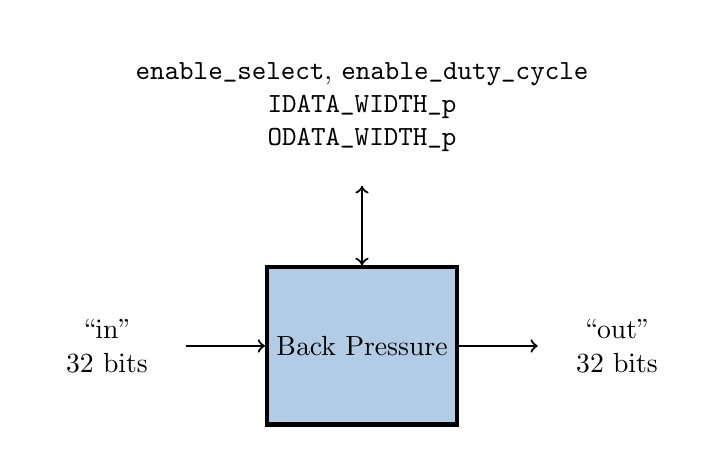
\begin{tikzpicture}[% List of styles applied to all, to override specify on a case-by-case
			every node/.style={
				align=center,  		% use this so that the "\\" for line break works
				minimum size=2cm	% creates space above and below text in rectangle
			},
			every edge/.style={draw,thick}
		]
		\node[rectangle,ultra thick,draw=black,fill=blue](R2){\Comp};
		\node[rectangle,draw=white,fill=white](R3)[left= of R2]{``in'' \\ 32 bits};
		\node[rectangle,draw=white,fill=white](R4)[right= of R2]{``out'' \\ 32 bits};
		\node[rectangle,draw=white,fill=white](R5)[above= of R2]{\verb+enable_select+, \verb+enable_duty_cycle+\\ \verb+IDATA_WIDTH_p+\\ \verb+ODATA_WIDTH_p+};
		\path[->]
		(R3)edge []	node [] {} (R2)
		(R2)edge []	node [] {} (R4)
		(R2)edge []	node [] {} (R5)
		(R5)edge []	node [] {} (R2)
		;
	\end{tikzpicture}
	\captionof{figure}{Top Level Block Diagram}
\end{center}\pagebreak

\subsection*{State Machine}
	N/A

\section*{Source Dependencies}
\subsection*{\comp.hdl}
\begin{itemize}
	\item projects/core/components/backpressure.hdl/backpressure.vhd
\end{itemize}

\subsection*{\comp.rcc}
\begin{itemize}
	\item projects/core/components/backpressure.rcc/backpressure.cc
\end{itemize}

\begin{landscape}
	\section*{Component Spec Properties}
	\begin{scriptsize}
		\begin{tabular}{|p{2cm}|p{1.5cm}|c|c|c|p{1.5cm}|p{1cm}|p{7cm}|}
			\hline
			\rowcolor{blue}
			Name                 & Type   & SequenceLength & ArrayDimensions & Accessibility       & Valid Range & Default & Usage                                                 \\
			\verb+enable_select+     & bool & -              & -               & Readable, Writable  & Standard    & False       & Select back pressure scheme to control 'take' from upstream worker. True = uses lfsr-15 or False = uses configurable duty cycle \\
			\hline
			\verb+enable_duty_cycle+   & ushort & -              & -               & Readable, Writable  & Standard    & 1    & Set 'take' duty cycle: 1 = constant, 2 = toggle, 3 = 1/on 2/off, 4 = 1/on 3/off, etc. \\
			\hline
		\end{tabular}
	\end{scriptsize}

	\section*{Worker Properties}
	\subsection*{\comp.hdl}
	\begin{scriptsize}
		\begin{tabular}{|p{2cm}|p{1.5cm}|c|c|c|p{1.5cm}|p{1cm}|p{7cm}|}
			\hline
			\rowcolor{blue}
			Name                      & Type  & SequenceLength & ArrayDimensions & Accessibility       & Valid Range & Default & Usage                                      \\
			\hline
			\verb+IDATA_WIDTH_p+ & ulong  & -              & -               & Readable, Parameter & 8/16/32/64  & 32      & Input port data width                                 \\
			\hline
			\verb+ODATA_WIDTH_p+ & ulong  & -              & -               & Readable, Parameter & 8/16/32/64  & 32      & Output port data width                                \\
			\hline
		\end{tabular}
	\end{scriptsize}

	\section*{Component Ports}
	\begin{scriptsize}
		\begin{tabular}{|M{2cm}|M{1.5cm}|M{4cm}|c|c|M{9cm}|}
			\hline
			\rowcolor{blue}
			Name & Producer & Protocol & Optional & Advanced & Usage                                  \\
			\hline
			in   & False    & -        & False    & -        & 32 bits                            \\
			\hline
			out  & True     & -        & False    & -        & 32 bits \\
			\hline
		\end{tabular}
	\end{scriptsize}

	\section*{Worker Interfaces}
	\subsection*{\comp.hdl}
	\begin{scriptsize}
		\begin{tabular}{|M{2cm}|M{1.5cm}|M{4cm}|c|M{12cm}|}
			\hline
			\rowcolor{blue}
			Type            & Name & DataWidth            & Advanced & Usage                                       \\
			\hline
			StreamInterface & in   & \verb+IDATA_WIDTH_p+ & -        & Size defined by \verb+IDATA_WIDTH_p+        \\
			\hline
			StreamInterface & out  & \verb+ODATA_WIDTH_p+ & -        & Sample size defined by \verb+ODATA_WIDTH_p+ \\
			\hline
		\end{tabular}
	\end{scriptsize}
\end{landscape}

\section*{Control Timing and Signals}
\subsection*{\comp.hdl}
\begin{flushleft}
	This worker implementation uses the clock from the Control Plane and standard Control Plane signals.
\end{flushleft}

\begin{landscape}
\section*{Worker Configuration Parameters}
\subsubsection*{\comp.hdl}
%\input{../../\ecomp.hdl/configurations.inc}
\section*{Performance and Resource Utilization}
\subsubsection*{\comp.hdl}
%\input{../../\ecomp.hdl/utilization.inc}
\end{landscape}

\section*{Test and Verification}
\begin{flushleft}
This component is tested via the unit test automation feature of the framework.  The component's .test/ contains XML files that describe the combinations of tests. \medskip

Fundamentally, there are two test cases that are employed to verify the Back Pressure component:

\begin{enumerate}
	\item enable\_select = True: The most significant bit of the lfsr-15 drives the 'take' signal of the input port.
	\item enable\_select = False: The enable\_duty\_cycle setting controls the duty cycle of the 'take' signal of the input port.
\end{enumerate}

	In all test cases, the data is simply passed through the worker and the tests are determined to be successful by comparing the input and output files. Due to its simplicity, and usage in other unit tests, a binary data file is generated containing complex signed 16-bit samples with a tone at a configurable center frequency and sample frequency. Plotting of the I/O data is available, via View=1, if desired.
\end{flushleft}
\end{document}
